%\newpage

\subsection{Specific Aim 3: Efficient high-order numerical methods for
large-scale simulations}
\label{subsec:specific_aim_3}
% ----------------------------------------------------------------------
The HAP model requires solving exterior Dirichlet problems for the
screened Laplace equation and the Stokes mobility problem at each time
step in complex domains such as in Figure~\ref{fig:domain}. If
discretizing these equations with stencil-based numerical methods, the
computational domain must be truncated, the fluid volume must be
discretized, and artificial boundary conditions must be imposed. The
artificial boundary conditions introduces additional error, and
discretizing the volume results in an excessively large linear system.
Moreover, it is difficult to obtain high-order discretizations when the
boundary surfaces are irregular. Alternatively, since we are solving
constant-coefficient elliptic PDEs, the solution of the PDE can be
represented as layer potentials
\begin{align}
  \label{eq:LP}
  u(x) = \int_{\partial\Omega} K(x,y) \sigma(y)\,ds_y,
\end{align}
where $\sigma$ is an unknown density function, and $K(x,y)$ is a
derivative of the fundamental solution of the underlying PDE. By
matching the boundary condition at $x_0 \in \partial\Omega$ with the
limit of equation~\eqref{eq:LP} as $x\rightarrow x_0$, a BIE for the
density function is formed. Numerical methods to solve BIEs have several
advantages over their PDE-based counterpart: by construction, the layer
potential~\eqref{eq:LP} satisfies far-field conditions; only
$\partial\Omega$ needs to be discretized; carefully chosen kernels
$K(x,y)$ result in a well-conditioned linear system that is solved with
a mesh-independent number of GMRES iterations; and high-order or
spectral accuracy is attainable with appropriate quadrature methods. In
our previous work~\cite{Fu2018_SIAM} we demonstrate that BIEs are a
powerful tool to simulate two-dimensional suspensions of amphiphilic
particles. In addition to improving two-dimensional simulations, we will
extend the results to three dimensions using a standard
three-dimensional BIE formulation of the screened Laplace
equation~\cite{ying_2006} and a well-conditioned BIE formulation of the
mobility problem~\cite{manasthesis, rac-gre2016}.

Significant challenges to solve BIEs include solving dense linear
systems, developing preconditioning strategies, and developing
quadrature methods for integrands that are nearly singular. These
challenges are described in section~\ref{subsec:NumericalIssues}.
However, numerical errors can still lead to unphysical contact between
bodies. We propose two algorithms to avoid contact in
Section~\ref{subsec:timeStepping}. Then, proposed work for
well-conditioned BIE formulations of fluctuating hydrodynamics are
described in Section~\ref{subsec:fluctuating}.


% ----------------------------------------------------------------------
\subsubsection{Numerical issues}
\label{subsec:NumericalIssues}

Discretizations of carefully chosen BIEs can be solved with a
mesh-independent number of GMRES
iterations~\cite{cam-ips-kel-mey-xue1996}. Therefore, the required CPU
time is proportional to the cost of a matrix-vector multiplication that
can be done in optimal or near-optimal time with the fast multipole
method (FMM)~\cite{fmm5} and its extensions~\cite{fmm1, fmm2, fmm3,
fmm4, fmm6, fmm7, fmm8}. PI Quaife is experienced with applying FMMs to
BIE formulations of the Stokes equation~\cite{qua-bir2014,
bys-sha-qua2020} and the screened Laplace equation~\cite{kro-qua2011,
qua2011}. Alternatively, fast direct solvers can be used to avoid
iteration~\cite{fds1, fds2, fds3, fds4, fds5, fds6, fds7, fds8,
ho2016cpam2, ho2016cpam1, minden2016, minden2017siammms}, but direct
solvers often require a large amount of initial overhead, and this makes
them less practical for problems with moving geometries. Alternatively,
techniques in fast direct solvers can be used to develop efficient
preconditioning strategies such as the inverse Fast Multipole Method
(IFMM)~\cite{cou-pou-dar2017}. PI Quaife used the IFMM to precondition
Stokes equations in a porous media~\cite{qua-cou-dar2018}, and a suite
of other preconditioners including sparse approximate
inverses~\cite{che2000} and multigrid~\cite{hem-sch1981, sch1982} will
be investigated.

\begin{wrapfigure}[21]{r}{3.0in}
%\vspace*{+15pt}
\centerline{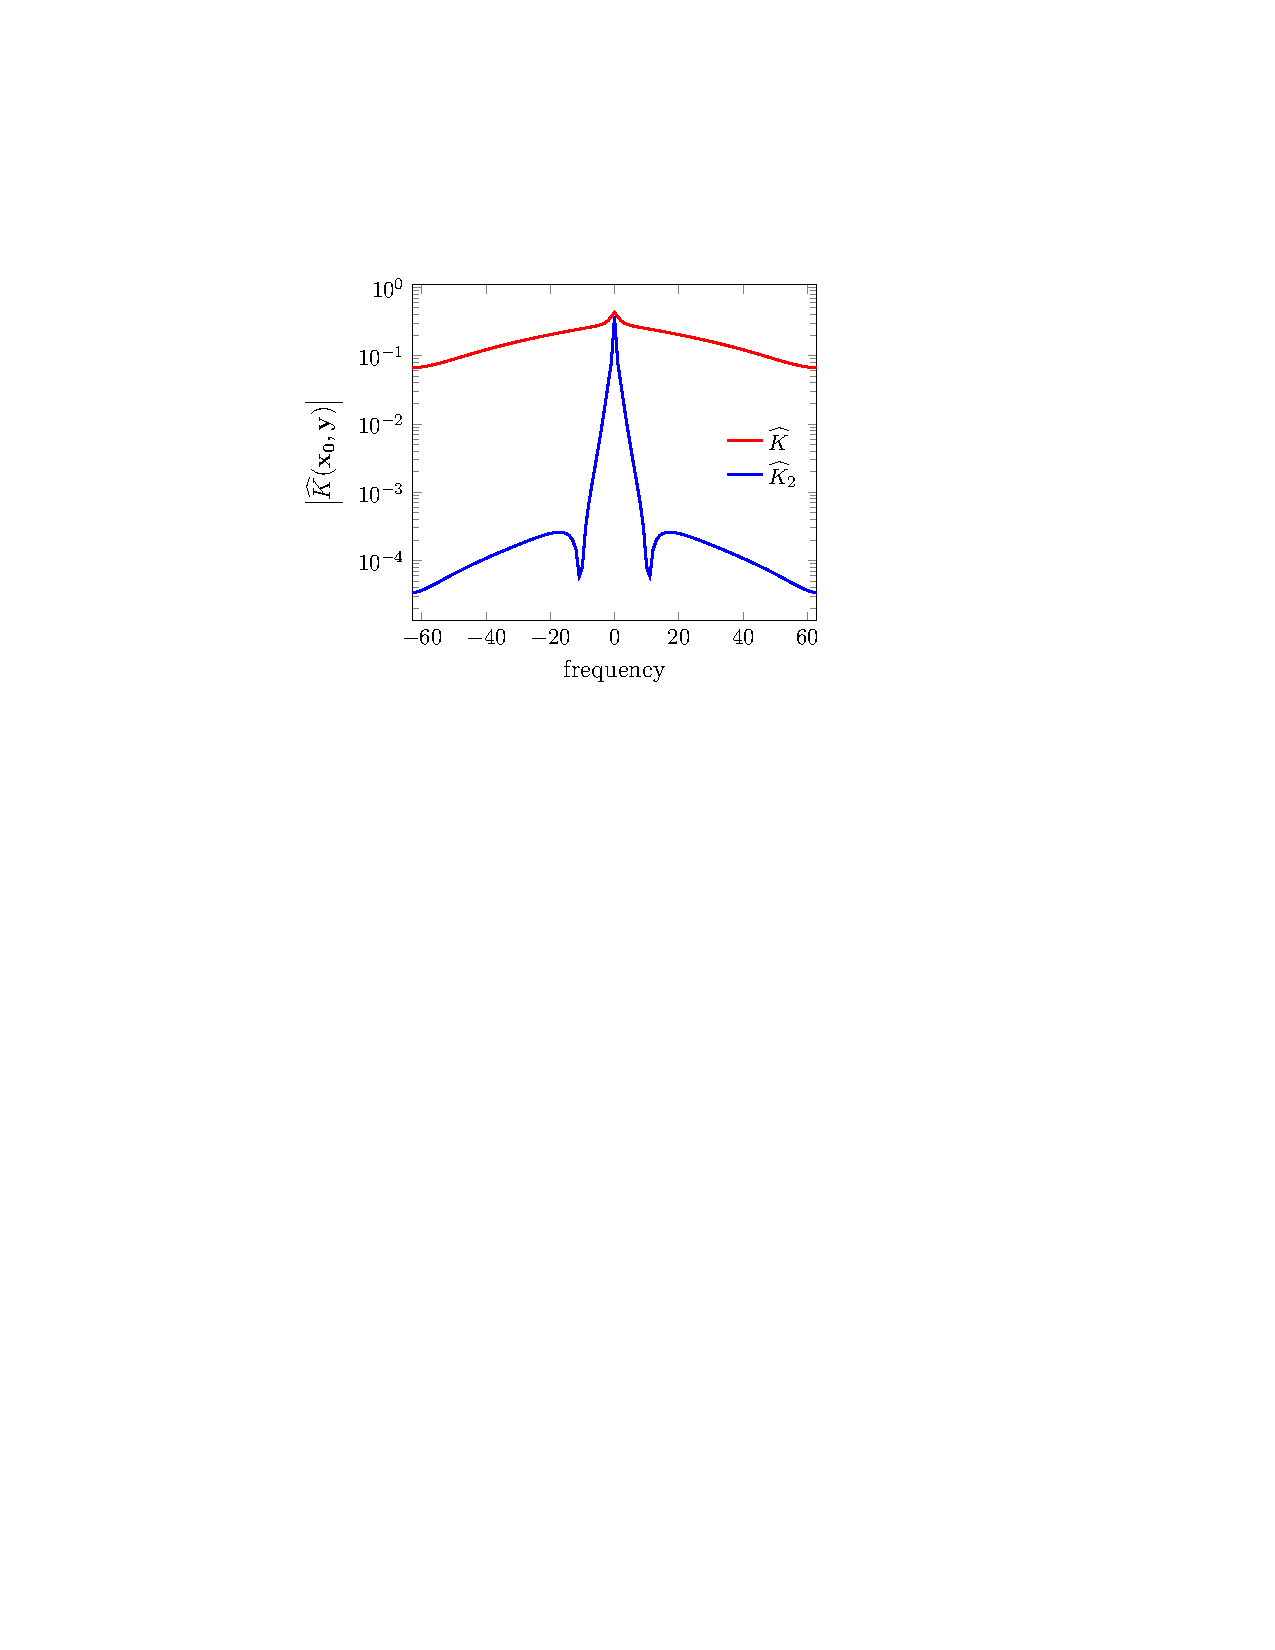
\includegraphics[width=3.0in]{figures/integrands}}
\vspace*{-13pt}
\caption{{\footnotesize The Fourier modes of $K(x_0,y)$ and $K_2(x_0,y)$
  where $\|x_0\| = 0.99$ and $y \in \partial\Omega$, where
  $\partial\Omega$ is the unit circle. The trapezoid rule applied to the
  red integrand has large amounts of error, but the trapezoid rule is
  much more accurate when applied to the blue integrand. Since the
  difference between the red and blue curves can be accurately computed
  with the barycentric quadrature rule, the quadrature error applied to
  layer potentials for the screen Laplace equation will be uniformly
  bounded in $\Omega$.}}
\label{fig:integrands}
\end{wrapfigure}
Nearly touching bodies is ubiquitous in self-assembly of amphiphilic
particles, and this results in nearly-singular integrands. Quadrature
methods for these integrands has received a lot of attention in
two and three dimensions~\cite{alpert, kapur, sidi, duffy, bruno1,
bruno2, davis_1984, graglia_2008, hackbusch_sauter_1994, jarvenpaa_2003,
khayat_2005, schwab_1992, ying_2006, beale1, beale2, goodman_1990,
haroldson_1998, lowengrub_1993, schwab_1992, ggq1, ggq2, ggq3,
helsing_2008a, helsing_integral_2009, helsing_tutorial_2012,
klockner2013jcp, qbx2, wala2019jcp, af2018sisc, siegel2018jcp,
rachh2017jcp, ding2019arxiv, bar2014}. The trapezoid rule is the
workhorse for two-dimensional BIEs since it achieves spectral accuracy
when integrands are not nearly-singular~\cite{tre-wei2014}. To address
nearly-singular integrands of two-dimensional BIEs, we will use a {\em
barycentric quadrature rule} that only requires a slight modification of
the trapezoid rule~\cite{ioa-pap-per1991}. This method requires the
layer potential satisfy Laplace or Stokes
equations~\cite{bar-wu-vee2015, chi-moo-qua2020}. The PIs will extend
this quadrature method to layer potentials for the screened Laplace
equation. This will be done by recognizing that the fundamental solution
of the screened Laplace equation can be decomposed as $K(x,y) = K_1(x,y)
+ K_2(x,y)$, where $K_1(x,y) = -\log\|x - y\|$ and $K_2(x,y) = K(x,y) +
\log\|x - y\|$. Using this decomposition, layer potentials involving
$K_1(x,y)$ can be accurately computed with the barycentric quadrature
rule~\cite{ioa-pap-per1991}, and layer potentials involving $K_2(x,y)$
can be accurately computed with the trapezoid rule since the kernel is
bounded for all $x$ and $y$. The proposed method is demonstrated in
Figure~\ref{fig:integrands} where the amplitude of the Fourier modes of
$K(x_0,y)$ and $K_2(x_0,y)$ are plotted. The quadrature of the trapezoid
rule is the sum of the Fourier amplitudes not captured at the
resolution.


% ----------------------------------------------------------------------
\subsubsection{Eliminating contact with adaptive time stepping and
repulsion}
\label{subsec:timeStepping}

A numerical issue when simulating the self-assembly of amphiphilic
particles is avoiding particle collision. The hydrophobic attraction
potential drives the amphiphilic particles towards one another so to
minimize exposure to the solvent, and this leads to physical contact in
finite time. Such particle collisions in a dense rigid body suspension
is a great challenge and can be a bottleneck in large-scale simulations.
We propose two algorithms to remedy this computational challenge:
high-order adaptive time stepping and repulsion forces.

PI Quaife developed a high-order adaptive time stepping method for
hydrodynamic suspensions~\cite{qua-bir2016} and it has served as a
robust method to simulate processes including mixing and adhesion in
suspensions~\cite{qua-vee-you2019, kab-qua-bir2017}. The method uses
a single-step high-order time stepping method and a computationally
cheap estimate of the error. The proposed work will use a spectral
deferred correction method~\cite{dut-gre-rok2000} since it iteratively
applies a low-order single-step method to achieve high-order accuracy.
To estimate the error, at each time step we will compute the total force
and torque of the system which is computationally cheap and physically
zero. The PIs' experience is that error estimates based on physical
constraints such as force- and torque-free conditions appropriately
adjust the time step size so that the dynamics are resolved without the
computational expense of techniques such as embedded Runge-Kutta
methods, step-doubling, and Richardson extrapolation.

Our previous work avoids contact by including a Leonard-Jones body
forces~\cite{Fu2018_SIAM}. Such a steep steric interaction at short
ranges introduces numerical stiffness and limits the time step size. To
remove this stiffness, we propose a geometry-based contact
method~\cite{har-pon-sor-zor2011}, and this method has been applied to
vesicle suspensions~\cite{lu-rah-zor2017} and rigid body suspensions in
two dimensions~\cite{bys-sha-qua2020} and three
dimensions~\cite{Yan2019}. These methods determine repulsion force by
solving a non-linear complementarity problem with a geometric constraint
that the configuration is non-overlapping.


% ----------------------------------------------------------------------
\subsubsection{Fluctuating hydrodynamics}
\label{subsec:fluctuating}
Once algorithms that address quadrature, adaptive time stepping, and
contact are implemented, we will embark on incorporating fluctuating
hydrodynamics that are important even at scales of the some amphiphilic
particles. Bao et al.~\cite{Bao17,Bao18} developed two-dimensional BIE
formulations for Brownian rigid bodies. To satisfy the covariance of the
rigid body velocities, an ill-conditioned first-kind integral equation
method is used. The proposed work will consider a double-layer potential
formulation that has much better conditioning properties. This strategy
was attempted in~\cite{Bao18}, but they claim that a necessary
regularization of the covariance matrix leads to a drastic loss of
accuracy in numerical fluctuation-dissipation balance. However, they
only one regularization strategy was considered, and as PI Quaife has
shown in previous work, the regularization choice significantly affects
the resulting physics~\cite{ong-chr-qua2017}. Therefore, different
regularization strategies will be investigated with the goal of
controlling the accuracy of the fluctuation-dissipation balance.


